\documentclass[t,aspectratio=169]{beamer}
%\usetheme{Berkeley}
\usepackage{graphicx}
\usepackage{amsmath}
\usepackage[american]{circuitikz}

\title{Clase 18}
\subtitle{El modelo re del BJT}
\author{Dr.-Ing. Juan José Montero Rodríguez}
\subject{Elementos Activos}
\institute{Escuela de Ingeniería Electrónica}
\date{Semestre II-2023}

\begin{document}

\begin{frame}{}
\maketitle
\end{frame}

\section{Emisor común}
\begin{frame}{Modelo re del transistor BJT en emisor común}

El transistor BJT NPN conectado en emisor común:

\begin{itemize}
    \item Entrada en la base ($V_{BE}$)
    \item Salida en el colector ($I_C$)
\end{itemize}

\begin{columns}
\begin{column}{0.33\textwidth}
\begin{figure}[H]
    \centering
    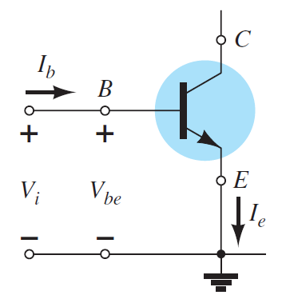
\includegraphics[width=0.8\textwidth]{figuras/modelo_re_ec_1.png}
\end{figure}
\end{column}
\begin{column}{0.33\textwidth}
\begin{figure}[H]
    \centering
    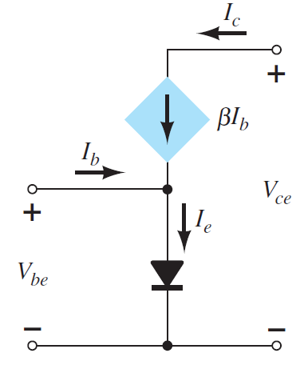
\includegraphics[width=0.8\textwidth]{figuras/modelo_re_ec_2.png}
\end{figure}
\end{column}
\begin{column}{0.33\textwidth}
\begin{figure}[H]
    \centering
    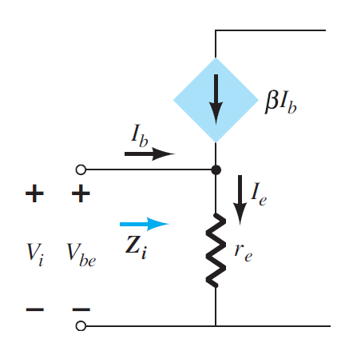
\includegraphics[width=0.8\textwidth]{figuras/modelo_re_ec_3.png}
\end{figure}
\end{column}
\end{columns}

\end{frame}


\begin{frame}{Modelo re del transistor BJT en emisor común}

Se puede separar la red de entrada y la red de salida:

\begin{figure}[H]
    \centering
    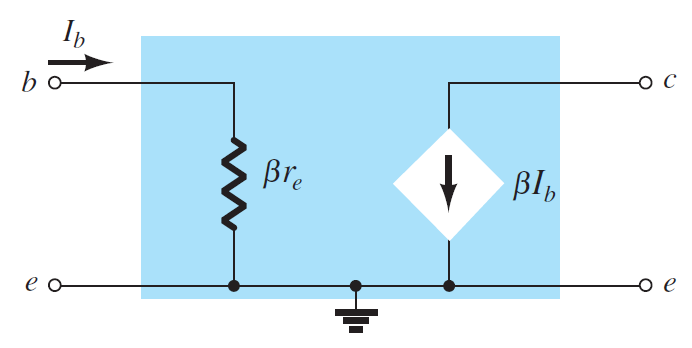
\includegraphics[width=0.6\textwidth]{figuras/modelo_re_ec_4.png}
\end{figure}

\[ r_e = \dfrac{V_t}{I_E} \]

\end{frame}


\begin{frame}{Inclusión de efecto Early}

\begin{columns}
\begin{column}{0.5\textwidth}
\begin{figure}[H]
    \centering
    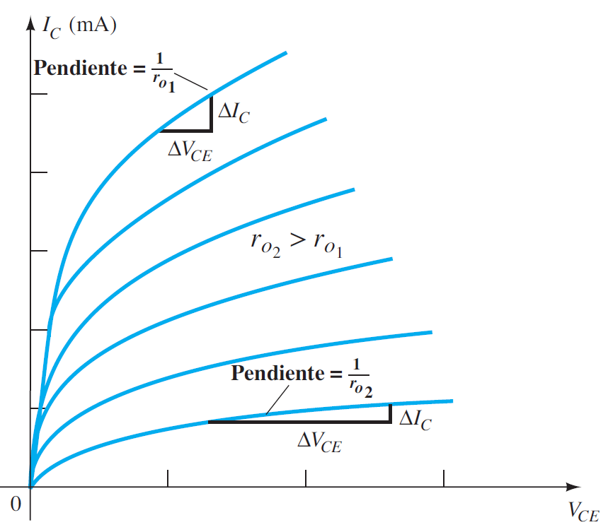
\includegraphics[width=\textwidth]{figuras/modelo_re_ec_5.png}
\end{figure}
\end{column}
\begin{column}{0.5\textwidth}
\begin{figure}[H]
    \centering
    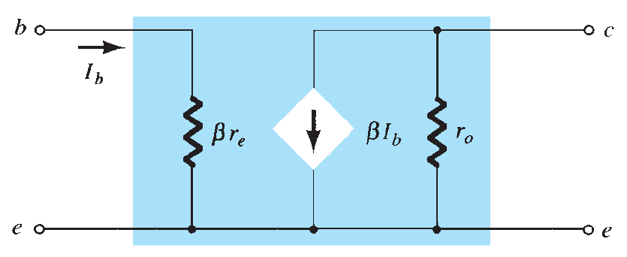
\includegraphics[width=\textwidth]{figuras/modelo_re_ec_6.png}
\end{figure}

\[ r_e = \dfrac{V_t}{I_E} \]
\[ r_o = \dfrac{V_A}{I_C} \]   

\end{column}
\end{columns}
    
\end{frame}


\section{Análisis EC}
\begin{frame}{Análisis de emisor común con modelo re}

\begin{columns}
\begin{column}{0.5\textwidth}
\begin{figure}[H]
    \centering
    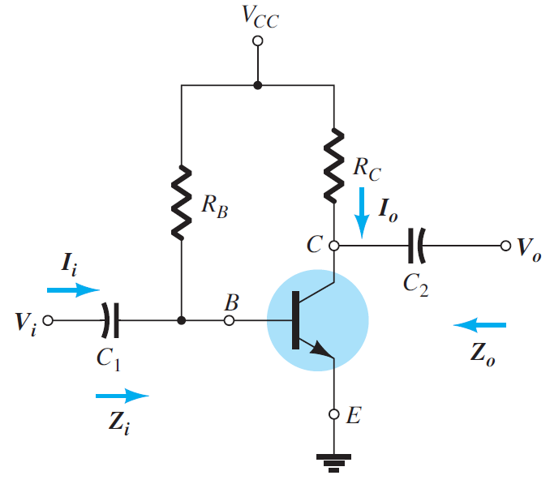
\includegraphics[width=\textwidth]{figuras/analisis_re_ec_1.png}
\end{figure}
\end{column}
\begin{column}{0.5\textwidth}
El equivalente en pequeña señal: 
\begin{itemize}
    \item Fuentes de CD apagadas
    \item Condensadores en corto
\end{itemize}

\begin{figure}[H]
    \centering
    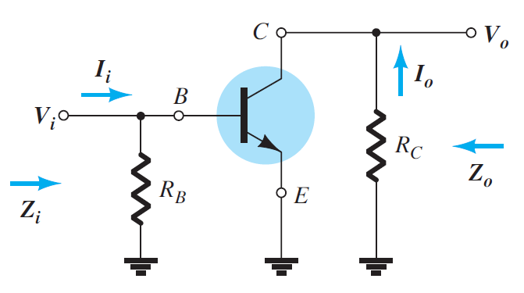
\includegraphics[width=\textwidth]{figuras/analisis_re_ec_2.png}
\end{figure}
\end{column}
\end{columns}

\end{frame}


\begin{frame}{Análisis de emisor común con modelo re}

Reemplazando el transistor por el modelo re:

\begin{figure}[H]
    \centering
    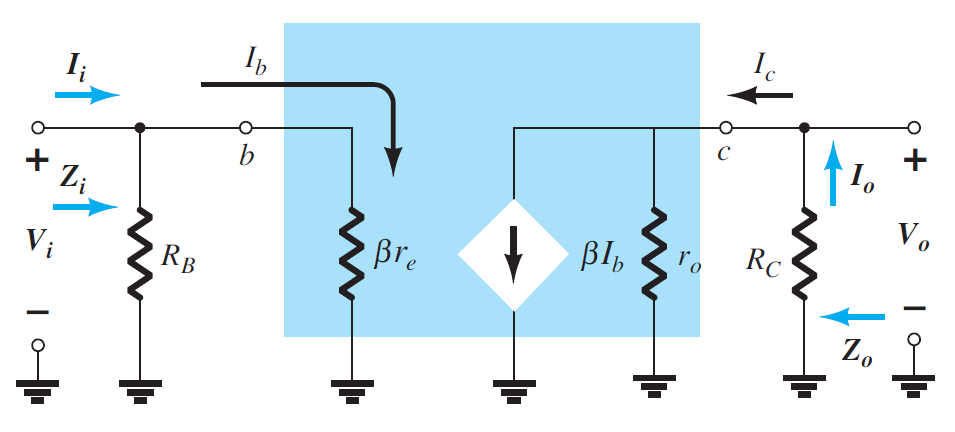
\includegraphics[width=\textwidth]{figuras/analisis_re_ec_3.png}
\end{figure}

\end{frame}


\begin{frame}{Análisis de emisor común con modelo re}

Reemplazando el transistor por el modelo re:

\begin{columns}
\begin{column}{0.6\textwidth}
\begin{figure}[H]
    \centering
    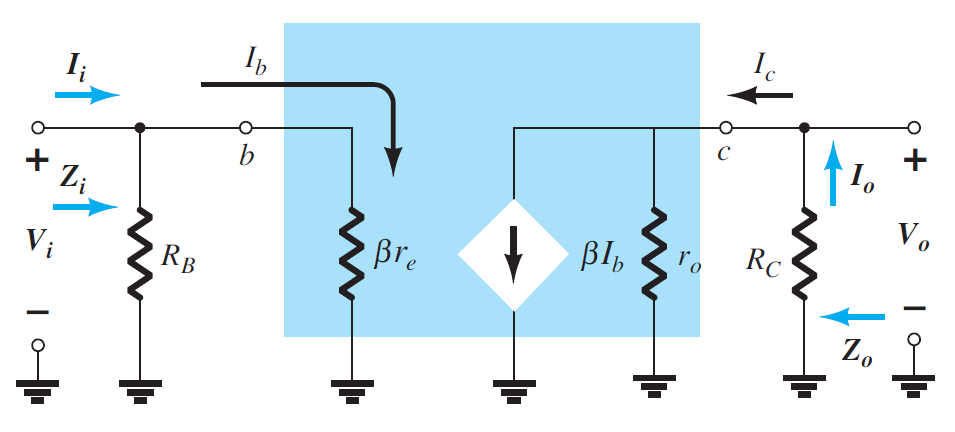
\includegraphics[width=\textwidth]{figuras/analisis_re_ec_3.png}
\end{figure}
\end{column}
\begin{column}{0.4\textwidth}
\[ V_o = -\beta I_b (R_C \parallel r_o) \]
\[ I_b = \dfrac{V_i}{\beta r_e} \]
\[ V_o = -\beta \left( \dfrac{V_i}{\beta r_e} \right) (R_C \parallel r_o) \]
\[ \boxed{A_V = \dfrac{V_o}{V_i} = -\dfrac{(R_C \parallel r_o)}{r_e} } \]
\end{column}
\end{columns}

\begin{columns}
\begin{column}{0.3\textwidth}
\[ \boxed{Z_i = R_B \parallel \beta r_e} \]
\end{column}
\begin{column}{0.3\textwidth}
\[ \boxed{Z_o = R_C \parallel r_o} \]
\end{column}
\begin{column}{0.4\textwidth}
\end{column}
\end{columns}

\end{frame}


\section{Ejemplo 1}
\begin{frame}{Ejemplo 1: Amplificador de emisor común}

Determine el punto de operación, la ganancia y las impedancias de entrada/salida del amplificador que se muestra en la figura, suponiendo que $V_{BE} = 0.7 V$.

\begin{figure}[H]
    \centering
    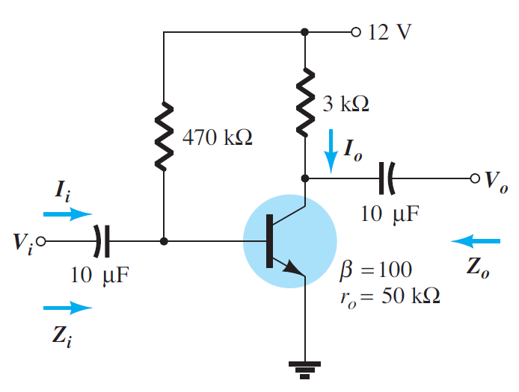
\includegraphics[width=0.5\textwidth]{figuras/ejemplo_1_circuito.png}
\end{figure}
    
\end{frame}


\begin{frame}{Solución 1: Amplificador de emisor común (gran señal)}

\begin{columns}
\begin{column}{0.5\textwidth}

\begin{figure}[H]
    \centering
    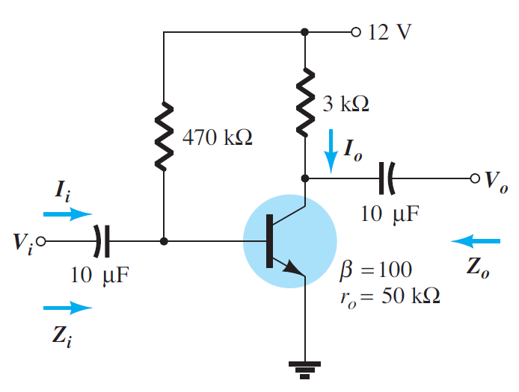
\includegraphics[width=\textwidth]{figuras/ejemplo_1_circuito.png}
\end{figure}

\end{column}
\begin{column}{0.5\textwidth}
\begin{align*}
&V_{BE} = 0.7\ V \\
&I_B = \dfrac{V_{CC} - V_{BE}}{R_B} = \dfrac{12\ V - 0.7\ V}{470\ k\Omega} = 24.04\ \mu A \\
&I_C = \beta I_B = (100)(24.04\ \mu A) = 2.404\ mA \\
&I_E = (\beta+1) I_B = (101)(24.04\ \mu A) = 2.428\ mA \\
&V_E = 0 \\
&V_B = V_{BE} = 0.7\ V \\
&V_C = V_{CC} - I_C R_C \\
&V_C = 5\ V - (2.404\ mA)(3\ k\Omega) = 4.788\ V \\
\end{align*}
%
¿Activa directa? $ V_C > V_B $

\end{column}
\end{columns}

\end{frame}


\begin{frame}{Solución 1: Amplificador de emisor común (pequeña señal)}

\begin{columns}
\begin{column}{0.5\textwidth}
%
\begin{figure}[H]
    \centering
    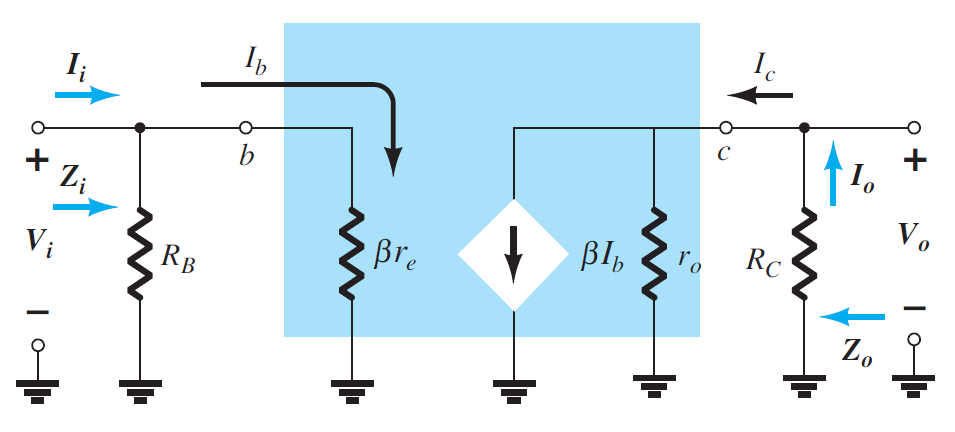
\includegraphics[width=\textwidth]{figuras/analisis_re_ec_3.png}
\end{figure}
%
\begin{align*}
&i_b = \dfrac{V_i}{\beta r_e} \\
&i_c = \beta \dfrac{V_i}{\beta r_e} \\
\end{align*}

\end{column}
\begin{column}{0.5\textwidth}
%
\begin{align*}
&v_{out} = -i_c R_C \\
&v_{out} = - \dfrac{V_i}{r_e} R_C \\
&\dfrac{v_{out}}{V_i} = - \dfrac{R_C}{r_e} \\
\end{align*}
%
\begin{align*}
&r_e = \dfrac{V_t}{I_E} = \dfrac{26\ mV}{2.428\ mV} = 10.708\ \Omega \\
&A_V = - \dfrac{R_C}{r_e} = - \dfrac{3\ k\Omega}{10.708\ \Omega} = -280.2 \\
\end{align*}

\end{column}
\end{columns}

\end{frame}


\section{Base común}
\begin{frame}{Modelo re del transistor BJT en base común}

El transistor BJT NPN conectado en base común:

\begin{itemize}
    \item Entrada en el emisor ($V_{BE}$)
    \item Salida en el colector ($I_C$)
\end{itemize}

\begin{columns}
\begin{column}{0.5\textwidth}

\begin{figure}[H]
    \centering
    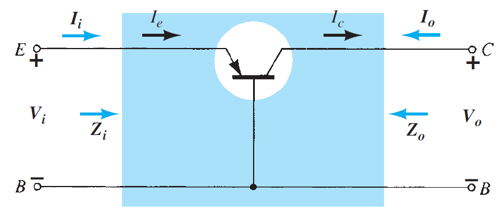
\includegraphics[width=\textwidth]{figuras/modelo_re_base_comun_1.png}
\end{figure}

\end{column}
\begin{column}{0.5\textwidth}

\begin{figure}[H]
    \centering
    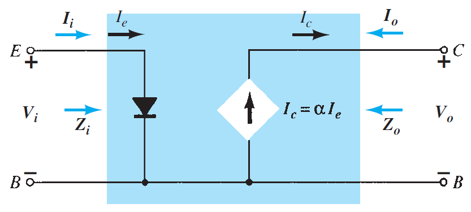
\includegraphics[width=\textwidth]{figuras/modelo_re_base_comun_2.png}
\end{figure}

\end{column}
\end{columns}

\end{frame}


\section{Ejemplo 2}
\begin{frame}{Ejemplo 2: Amplificador de base común}

Determine el punto de operación, la ganancia y las impedancias de entrada/salida del amplificador que se muestra, suponiendo que $V_{EB} = 0.7\ V$. Utilice el modelo $r_e$.

\begin{figure}[H]
    \centering
    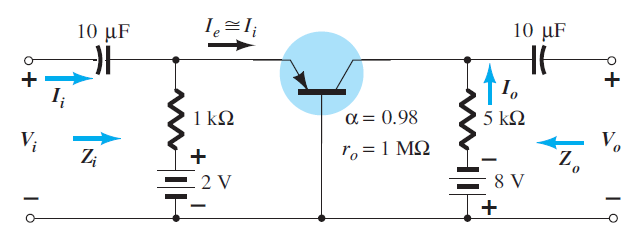
\includegraphics[width=\textwidth]{figuras/modelo_re_base_comun_3.png}
\end{figure}

\end{frame}


\begin{frame}{Solución 2: Amplificador de base común (gran señal)}

\begin{columns}
\begin{column}{0.5\textwidth}

\begin{figure}[H]
    \centering
    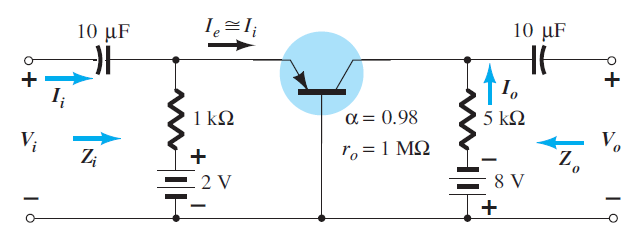
\includegraphics[width=\textwidth]{figuras/modelo_re_base_comun_3.png}
\end{figure}

\end{column}
\begin{column}{0.5\textwidth}

\begin{align*}
&V_{EB} = 0.7\ V \\
&I_E = \dfrac{V_{EE} - V_{EB}}{R_E} = \dfrac{2\ V - 0.7\ V}{1\ k\Omega} = 1.3\ mA \\
&I_C = \alpha I_E = (0.98)(1.3\ mA) = 1.274\ mA \\
&\beta = \dfrac{\alpha}{1 - \alpha} = \dfrac{0.98}{1 - 0.98} = 49 \\
&I_B = \dfrac{I_C}{\beta} = \dfrac{1.274\ mA}{49} = 26\ \mu A \\
\end{align*}

\end{column}
\end{columns}

\end{frame}


\begin{frame}{Solución 2: Amplificador de base común (pequeña señal)}

\begin{columns}
\begin{column}{0.5\textwidth}

\begin{figure}[H]
    \centering
    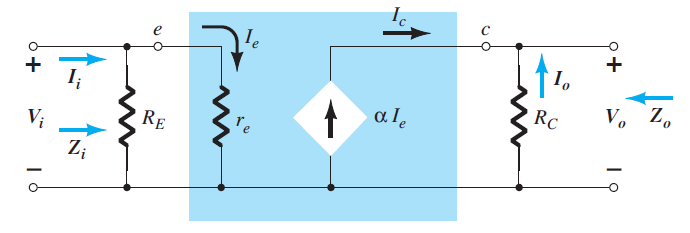
\includegraphics[width=\textwidth]{figuras/modelo_re_base_comun_4.png}
\end{figure}
%
\begin{align*}
&r_e = \dfrac{V_t}{I_E} = \dfrac{26\ mV}{1.3\ mA} = 20\ \Omega \\
&A_V = \dfrac{R_C}{r_e} = \dfrac{5\ k\Omega}{20\ \Omega} = 250 \\
&Z_i = R_E \parallel r_e = 1\ k\Omega \parallel 20\ \Omega = 19.61\ \Omega \\
&Z_o = R_C = 5\ k\Omega \\
\end{align*}

\end{column}
\begin{column}{0.5\textwidth}
\begin{align*}
&\boxed{Z_i = R_E \parallel r_e} \\
&\boxed{Z_o = R_C} \\
& \\
&V_o = -I_o R_C = -(-I_C)R_C = \alpha I_E R_C \\
&I_e = \dfrac{V_i}{r_e} \\
&V_o = \alpha \left( \dfrac{V_i}{r_e} \right) R_C \\
&\boxed{A_V = \dfrac{V_o}{V_i} = \dfrac{\alpha R_C}{r_e} \approx \dfrac{R_C}{r_e}} \\
\end{align*}
\end{column}
\end{columns}

\end{frame}


\section{Colector común}
\begin{frame}{Modelo re del transistor BJT en colector común (seguidor de emisor)}

\begin{columns}
\begin{column}{0.5\textwidth}

\begin{figure}[H]
    \centering
    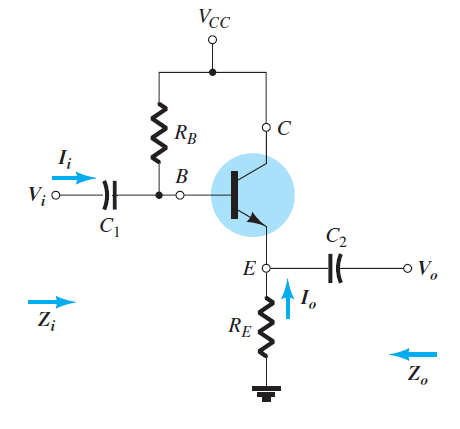
\includegraphics[width=\textwidth]{figuras/modelo_re_colector_comun_1.png}
\end{figure}

\end{column}
\begin{column}{0.5\textwidth}

\begin{figure}[H]
    \centering
    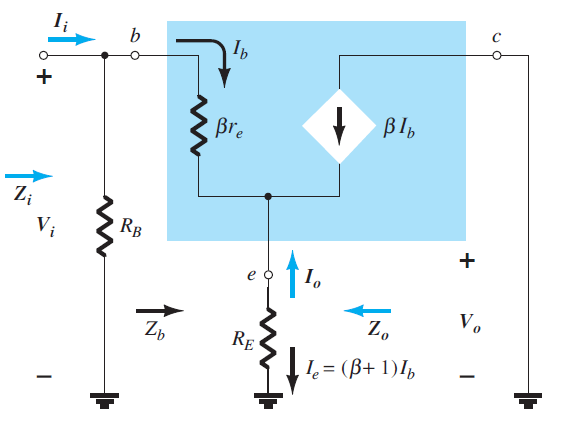
\includegraphics[width=\textwidth]{figuras/modelo_re_colector_comun_2.png}
\end{figure}

\end{column}
\end{columns}

\end{frame}


\begin{frame}{Análisis de colector común con modelo re}

\begin{columns}
\begin{column}{0.5\textwidth}

\begin{figure}[H]
    \centering
    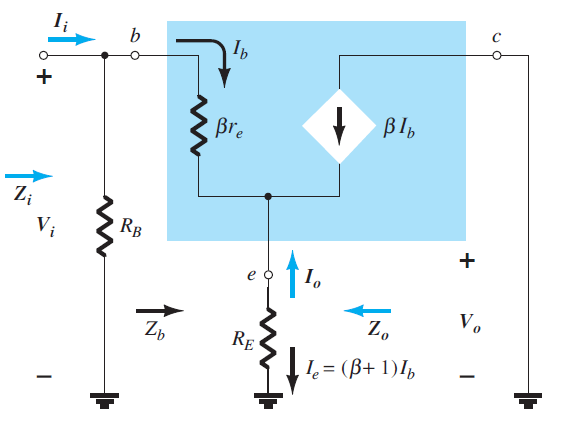
\includegraphics[width=\textwidth]{figuras/modelo_re_colector_comun_2.png}
\end{figure}

\end{column}
\begin{column}{0.5\textwidth}

\begin{align*}
&\boxed{Z_i = R_B \parallel Z_b} \\
&\boxed{Z_b = \beta r_e + (\beta + 1) R_E} \\
&\boxed{Z_o = R_E \parallel r_e} \\
&\boxed{A_V = \dfrac{V_o}{V_i} = \dfrac{R_E}{R_E + r_e}} \\
\end{align*}

\end{column}
\end{columns}

\end{frame}


\section{Ejemplo 3}
\begin{frame}{Ejemplo 3: Amplificador de colector común}

Para el circuito en emisor seguidor mostrado en la figura, determine el punto de operación y calcule la ganancia y las impedancias de entrada/salida.

\begin{figure}[H]
    \centering
    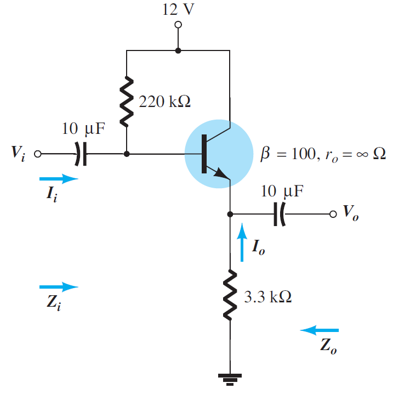
\includegraphics[width=0.45\textwidth]{figuras/modelo_re_colector_comun_3.png}
\end{figure}

\end{frame}


\begin{frame}{Solución 3: Amplificador de colector común (gran señal)}

\vspace{-5mm}
\begin{columns}
\begin{column}{0.4\textwidth}
%
\begin{figure}[H]
    \centering
    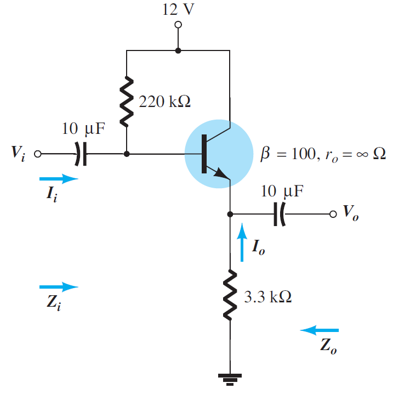
\includegraphics[width=\textwidth]{figuras/modelo_re_colector_comun_3.png}
\end{figure}
%
\end{column}
\begin{column}{0.6\textwidth}
%
\begin{align*}
&V_{BE} = 0.7\ V \\
&V_{CC} = I_B R_B + V_{BE} + I_E R_E \\
&V_{CC} = I_B R_B + V_{BE} + (\beta + 1) I_B R_E \\
&I_B = \dfrac{V_{CC} - V_{BE}}{R_B + (\beta + 1) R_E} \\
&I_B = \dfrac{12\ V - 0.7\ V}{220\ k\Omega + (101) (3.3\ k\Omega)} = 20.42\ \mu A \\
&I_C = \beta I_B = (100)(20.42\ \mu A) = 2.042\ mA \\
&I_E = (\beta + 1) I_B = (101)(20.42\ \mu A) = 2.062\ mA \\
&V_C = 12\ V \\
&V_B = V_{CC} - I_B R_B = 12\ V - (20.42\ \mu A)(220\ k\Omega) = 7.508\ V \\
&V_E = V_B - 0.7\ V = 6.808\ V \\
\end{align*}

\end{column}
\end{columns}

\end{frame}





\begin{frame}{Solución 3: Amplificador de colector común (pequeña señal)}

\begin{columns}
\begin{column}{0.5\textwidth}

\begin{figure}[H]
    \centering
    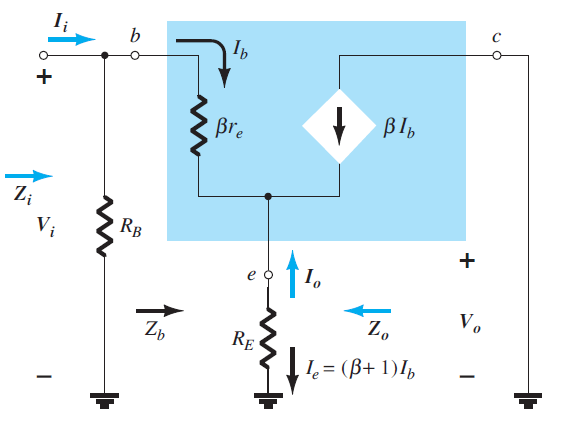
\includegraphics[width=\textwidth]{figuras/modelo_re_colector_comun_2.png}
\end{figure}

\end{column}
\begin{column}{0.5\textwidth}
\begin{align*}
&r_e = \dfrac{V_t}{I_E} = \dfrac{26\ mV}{2.062\ mV} = 12.61\ \Omega \\
&Z_b = \beta r_e + (\beta + 1) R_E \\
&Z_b = (100)(12.61\ \Omega) + (101)(3.3\ k\Omega) \\
&Z_b = 334.56\ k\Omega \\
&Z_i = R_B \parallel Z_b = 220\ k\Omega \parallel 334.56\ k\Omega \\
&Z_i = 132.72\ k\Omega \\
&Z_o = R_E \parallel r_e = 3.3\ k\Omega \parallel 12.61\ \Omega \\
&Z_o = 12.56\ \Omega \\
&A_V = \dfrac{V_o}{V_i} = \dfrac{R_E}{R_E + r_e} = \dfrac{3.3\ k\Omega}{3.3\ k\Omega + 12.61\ \Omega} \\
&A_V = 0.996 \\
\end{align*}

\end{column}
\end{columns}

\end{frame}


\section{Referencias}
\begin{frame}{Lecturas recomendadas}

\begin{itemize}
\item Boylestad, R. y Nashelsky, L. (2009). Electrónica: Teoría de Circuitos y Dispositivos Electrónicos. Capítulo 5: Análisis de ca de un BJT, pp. 246-254, Pearson Educación, México.
\end{itemize}

\end{frame}



\end{document}
